\section{Experiments}\label{sec:results}

This section describes the experimental setup, compares WaveletMask with state-of-the-art methods on synthetic and real-world data, presents the ablation study, and analyzes computational complexity. Detailed statistical-reliability analyses, robustness and cross-content generalization studies, detector diagnostic probes, and full ablation sweeps are reported in Appendices~\ref{app:stats}--\ref{app:complexity_details}.

\subsection{Datasets}

Experiments are conducted on the Synthetic and Real-World Old Video (SRWOV) benchmark introduced with MambaOFR~\cite{mao2025mambaofr}. The synthetic split provides paired ground truth and is used for full-reference evaluation. The real-world split contains archival clips without paired ground truth and is used for no-reference metrics and qualitative comparisons.

Training uses the REDS training split~\cite{nah2019reds}. Clean REDS frames are degraded on the fly with the synthetic film degradation pipeline used by RTN~\cite{rtn2022}, including scratches, dust, blotches, flicker, and grain. The SRWOV synthetic test set contains 30 clips rendered from held-out REDS sequences, and the SRWOV real-world set contains 216 archival clips. Unless otherwise noted, the quantitative results below are reported within this SRWOV protocol. Qualitative figures are illustrative; statistical claims rest on the unified re-training benchmark in Table~\ref{tab:literature_context} and the strict paired controlled analysis in Appendix~\ref{app:stats}.

\subsection{Implementation Details}\label{subsec:implementation}

RTN and all WaveletMask variants are trained with the same recipe. We use Adam~\cite{kingma2015adam} with $\beta_1=0.9$, $\beta_2=0.99$, initial learning rate $2\times10^{-4}$, and a MultiStep schedule with milestones at 50K, 100K, and 150K iterations. Training uses 200K iterations, seven input frames, $256\times256$ crops, and batch size~1 per GPU. The configuration sets \texttt{fix\_flow\_iters}=0.0005, so the RAFT~\cite{teed2020raft} optical-flow estimator is effectively trained jointly from the start rather than frozen for a 500-iteration warm-up. Experiments are implemented in PyTorch with the BasicSR toolbox~\cite{wang2022basicsr}; inference is performed at full resolution. The strict paired controlled comparison against the RTN (Appendix~\ref{app:stats}) is reported for seed 2021, and a three-seed Y-channel re-test is reported separately to assess seed stability.

\subsection{Evaluation Metrics}\label{subsec:metrics}

Following common practice in old film restoration~\cite{rtn2022,rrtn2024,mao2025mambaofr}, we adopt three complementary groups of metrics. (1) On the synthetic split with paired ground truth, we report the fidelity metrics PSNR and SSIM~\cite{wang2004ssim} together with the perceptual metrics LPIPS~\cite{zhang2018lpips} and DISTS~\cite{ding2020dists}; all full-reference metrics are computed under the Y-channel protocol. (2) On the real-world split without ground truth, we report the no-reference metrics NIQE~\cite{mittal2013niqe}, BRISQUE~\cite{mittal2012brisque}, and CLIPIQA+~\cite{wang2023clipiqa}; these no-reference metrics, together with the qualitative comparisons, constitute the primary real-world evidence. (3) To quantify statistical reliability, we report clip-level bootstrap confidence intervals, two-sided paired permutation tests, and a three-seed re-test for the paired controlled comparison; the complete statistics are provided in Appendix~\ref{app:stats}.

For completeness, the two primary full-reference metrics are defined as follows. Given a restored luminance frame $\hat{I}$ and its ground truth $I$ with $N$ pixels, the peak signal-to-noise ratio (PSNR) is
\begin{equation}
\mathrm{PSNR}(\hat{I}, I) = 10\log_{10}\frac{L^{2}}{\frac{1}{N}\sum_{i=1}^{N}(\hat{I}_{i}-I_{i})^{2}},
\end{equation}
where $L$ is the maximum possible pixel value, and the structural similarity index (SSIM) is
\begin{equation}
\mathrm{SSIM}(\hat{I}, I) = \frac{(2\mu_{\hat{I}}\mu_{I}+c_{1})(2\sigma_{\hat{I}I}+c_{2})}{(\mu_{\hat{I}}^{2}+\mu_{I}^{2}+c_{1})(\sigma_{\hat{I}}^{2}+\sigma_{I}^{2}+c_{2})},
\end{equation}
where $\mu_{\cdot}$ and $\sigma_{\cdot}$ denote local means and standard deviations, $\sigma_{\hat{I}I}$ is the local covariance, and $c_{1},c_{2}$ are small stabilizing constants. The perceptual metrics LPIPS and DISTS and the no-reference metrics NIQE, BRISQUE, and CLIPIQA+ follow the definitions in their original references.

\subsection{Comparison with State-of-the-Art Methods}\label{subsec:sota}

We compare WaveletMask with representative methods from three categories: old photo restoration applied per frame (OldPhoto~\cite{wan2020bringing}, DeOldify~\cite{jantic2019deoldify}), general video restoration (ShiftNet~\cite{li2023shiftnet}, VRT~\cite{liang2024vrt}, RVRT~\cite{liang2022rvrt}), and dedicated old film restoration (DeepRemaster~\cite{iizuka2019deepremaster}, RTN~\cite{rtn2022}, RRTN~\cite{rrtn2024}, MambaOFR~\cite{mao2025mambaofr}). All ten methods, including WaveletMask, were re-trained and re-evaluated on the same SRWOV synthetic split under one unified benchmark pipeline, so they are directly comparable; in addition, a strict paired controlled analysis against RTN---which shares the backbone, training data, degradation pipeline, and metric scripts with WaveletMask---is reported in Appendix~\ref{app:stats}.

\subsubsection{Quantitative Comparison on Synthetic Data}\label{subsec:sota_quant}

\begin{table}[H]
\caption{Unified re-training benchmark on the SRWOV synthetic split (30 clips, Y-channel protocol), listed in chronological order of publication with the proposed WaveletMask in the last row. All methods, including WaveletMask, were re-trained and re-evaluated by us under one unified benchmark pipeline, so the rows are directly comparable. Best results are in \textcolor{red}{red} and second-best results in \textcolor{blue}{blue}.\label{tab:literature_context}}
\footnotesize
\begin{tabularx}{\textwidth}{lcCCCC}
\toprule
\textbf{Method} & \textbf{Year} & \textbf{PSNR$\uparrow$} & \textbf{SSIM$\uparrow$} & \textbf{LPIPS$\downarrow$} & \textbf{DISTS$\downarrow$} \\
\midrule
DeepRemaster~\cite{iizuka2019deepremaster}  & 2019 & 25.0590 & \textcolor{red}{0.9185} & 0.1108 & 0.0895 \\
DeOldify~\cite{jantic2019deoldify}          & 2019 & 23.2197 & 0.8923 & 0.2775 & 0.1260 \\
OldPhoto~\cite{wan2020bringing}             & 2020 & 24.6174 & 0.8524 & 0.2252 & 0.1144 \\
RTN~\cite{rtn2022}                          & 2022 & 25.8514 & 0.8869 & 0.1214 & 0.0862 \\
RVRT~\cite{liang2022rvrt}                   & 2022 & 22.4317 & 0.8710 & 0.1655 & 0.1078 \\
ShiftNet~\cite{li2023shiftnet}              & 2023 & 21.4817 & 0.8234 & 0.2030 & 0.1303 \\
RRTN~\cite{rrtn2024}                        & 2024 & 24.1450 & 0.9006 & 0.1082 & \textcolor{red}{0.0668} \\
VRT~\cite{liang2024vrt}                     & 2024 & 22.3866 & 0.8631 & 0.1750 & 0.1087 \\
MambaOFR~\cite{mao2025mambaofr}             & 2025 & \textcolor{blue}{25.9938} & \textcolor{blue}{0.9059} & \textcolor{red}{0.0815} & \textcolor{blue}{0.0822} \\
\midrule
\textbf{WaveletMask (ours)}                 & 2026 & \textcolor{red}{26.6017} & 0.8951 & \textcolor{blue}{0.0891} & 0.0831 \\
\bottomrule
\end{tabularx}
\normalsize
\end{table}

Table~\ref{tab:literature_context} reports the unified re-training benchmark over ten methods. Under this single comparable protocol, WaveletMask attains the best PSNR (26.60~dB, $+0.61$~dB over the strongest competitor MambaOFR) and the second-best LPIPS. On DISTS it is essentially tied with the second-best method (0.0831 vs.\ 0.0822 for MambaOFR), whereas on SSIM it sits mid-table, behind the perception-oriented methods DeepRemaster, MambaOFR, and RRTN. The benchmark thus indicates a clear fidelity advantage together with competitive perceptual quality rather than uniform dominance across metrics: among the recent dedicated baselines, MambaOFR remains the strongest on the structural and perceptual scores, while WaveletMask leads on PSNR at a fraction of the detector parameter cost (Section~\ref{subsec:complexity}). Beyond this benchmark, a strict paired controlled comparison against the RTN isolates the contribution of the proposed gate: WaveletMask improves PSNR by $+0.45$~dB, all four paired clip-level gains are statistically significant under two-sided permutation tests ($p\le1.5\times10^{-3}$), and a three-seed re-test confirms that the advantage persists with markedly higher stability than the baseline (26.22$\pm$0.37 vs. 24.56$\pm$1.67~dB PSNR; Appendix~\ref{app:stats}, Tables~\ref{tab:same_protocol_main}--\ref{tab:three_seed_summary}). The WaveletMask unified-benchmark entry (26.6017~dB) differs slightly from this paired value (26.6125~dB), and the unified-benchmark RTN entry (25.8514~dB) likewise differs from the paired-protocol RTN (26.1648~dB; Table~\ref{tab:ablation_core}), because the two protocols use different training checkpoints and metric configurations. The gain is not confined to a single degradation mode: it is positive in all artifact-dominant strata, remains stable across motion and occlusion terciles, and transfers to unseen DAVIS content in PSNR, LPIPS, and DISTS under the same degradation pipeline (Appendix~\ref{app:robustness}).

\subsubsection{No-Reference Comparison on Real-World Data}\label{subsec:realworld}

Real-world SRWOV clips do not have paired ground truth, so we report them separately from the full-reference synthetic results. Table~\ref{tab:realworld_literature} reports our unified-benchmark no-reference scores for all ten methods together with the degraded-input anchor on the 216-clip SRWOV real-world split. A no-reference ablation over the RTN/LHFM/GFM variants under the strict paired protocol (Appendix~\ref{app:stats}) is provided in Appendix~\ref{app:complexity_details} (Table~\ref{tab:realworld_variants}).

\begin{table}[H]
\caption{No-reference evaluation on the 216-clip SRWOV real-world split. All values are measured by us under the unified benchmark pipeline; the degraded-input row is the unrestored anchor scored with the same per-frame protocol. Best results among the restoration methods are in \textcolor{red}{red} and second-best in \textcolor{blue}{blue}; the degraded-input anchor is excluded from ranking.\label{tab:realworld_literature}}
\footnotesize
\begin{tabularx}{\textwidth}{lCCC}
\toprule
\textbf{Method} & \textbf{NIQE$\downarrow$} & \textbf{BRISQUE$\downarrow$} & \textbf{CLIPIQA+$\uparrow$} \\
\midrule
Degraded input                              & 5.7745 & 43.1050 & 0.3873 \\
DeOldify~\cite{jantic2019deoldify}          & 5.7218 & 41.6118 & 0.3768 \\
DeepRemaster~\cite{iizuka2019deepremaster}  & 5.9917 & 40.6158 & 0.3991 \\
OldPhoto~\cite{wan2020bringing}             & 6.5601 & 30.4532 & \textcolor{red}{0.4503} \\
RTN~\cite{rtn2022}                          & \textcolor{red}{5.1723} & \textcolor{red}{19.0031} & 0.4163 \\
VRT~\cite{liang2024vrt}                     & 5.6551 & 42.7296 & 0.3985 \\
RVRT~\cite{liang2022rvrt}                   & 5.7217 & 42.6402 & 0.4013 \\
ShiftNet~\cite{li2023shiftnet}              & 5.7126 & 42.8195 & 0.3975 \\
RRTN~\cite{rrtn2024}                        & 5.6664 & 32.8572 & 0.3969 \\
MambaOFR~\cite{mao2025mambaofr}             & 5.3381 & 29.7853 & 0.4351 \\
\midrule
\textbf{WaveletMask (ours)}                 & \textcolor{blue}{5.2288} & \textcolor{blue}{24.2023} & \textcolor{blue}{0.4356} \\
\bottomrule
\end{tabularx}
\normalsize
\end{table}

In Table~\ref{tab:realworld_literature}, the ranking is mixed across NIQE, BRISQUE, and CLIPIQA+, which is expected for content-dependent no-reference metrics: the RTN checkpoint attains the best NIQE and BRISQUE, OldPhoto attains the best CLIPIQA+, and WaveletMask ranks second on all three metrics---the only method placing within the top two on every no-reference dimension, although its CLIPIQA+ margin over MambaOFR is narrow (0.4356 vs.\ 0.4351). Restoration clearly improves NIQE and BRISQUE over the degraded-input anchor for the strongest methods, yet individual no-reference metrics disagree on the absolute ranking, and the scores are sensitive to the training checkpoint: the paired-protocol RTN checkpoint in Appendix~\ref{app:complexity_details} (Table~\ref{tab:realworld_variants}) receives a clearly different BRISQUE score. The no-reference scores are therefore interpreted jointly with the qualitative comparisons below rather than as a standalone ranking. As an additional perceptual assessment on the real-world clips, an expert-level subjective evaluation is reported in the Supplementary Materials (Tables~S1 and~S2 and Figure~S4).

\subsubsection{Qualitative Comparison}\label{subsec:sota_qual}

\begin{figure}[t]
\centering
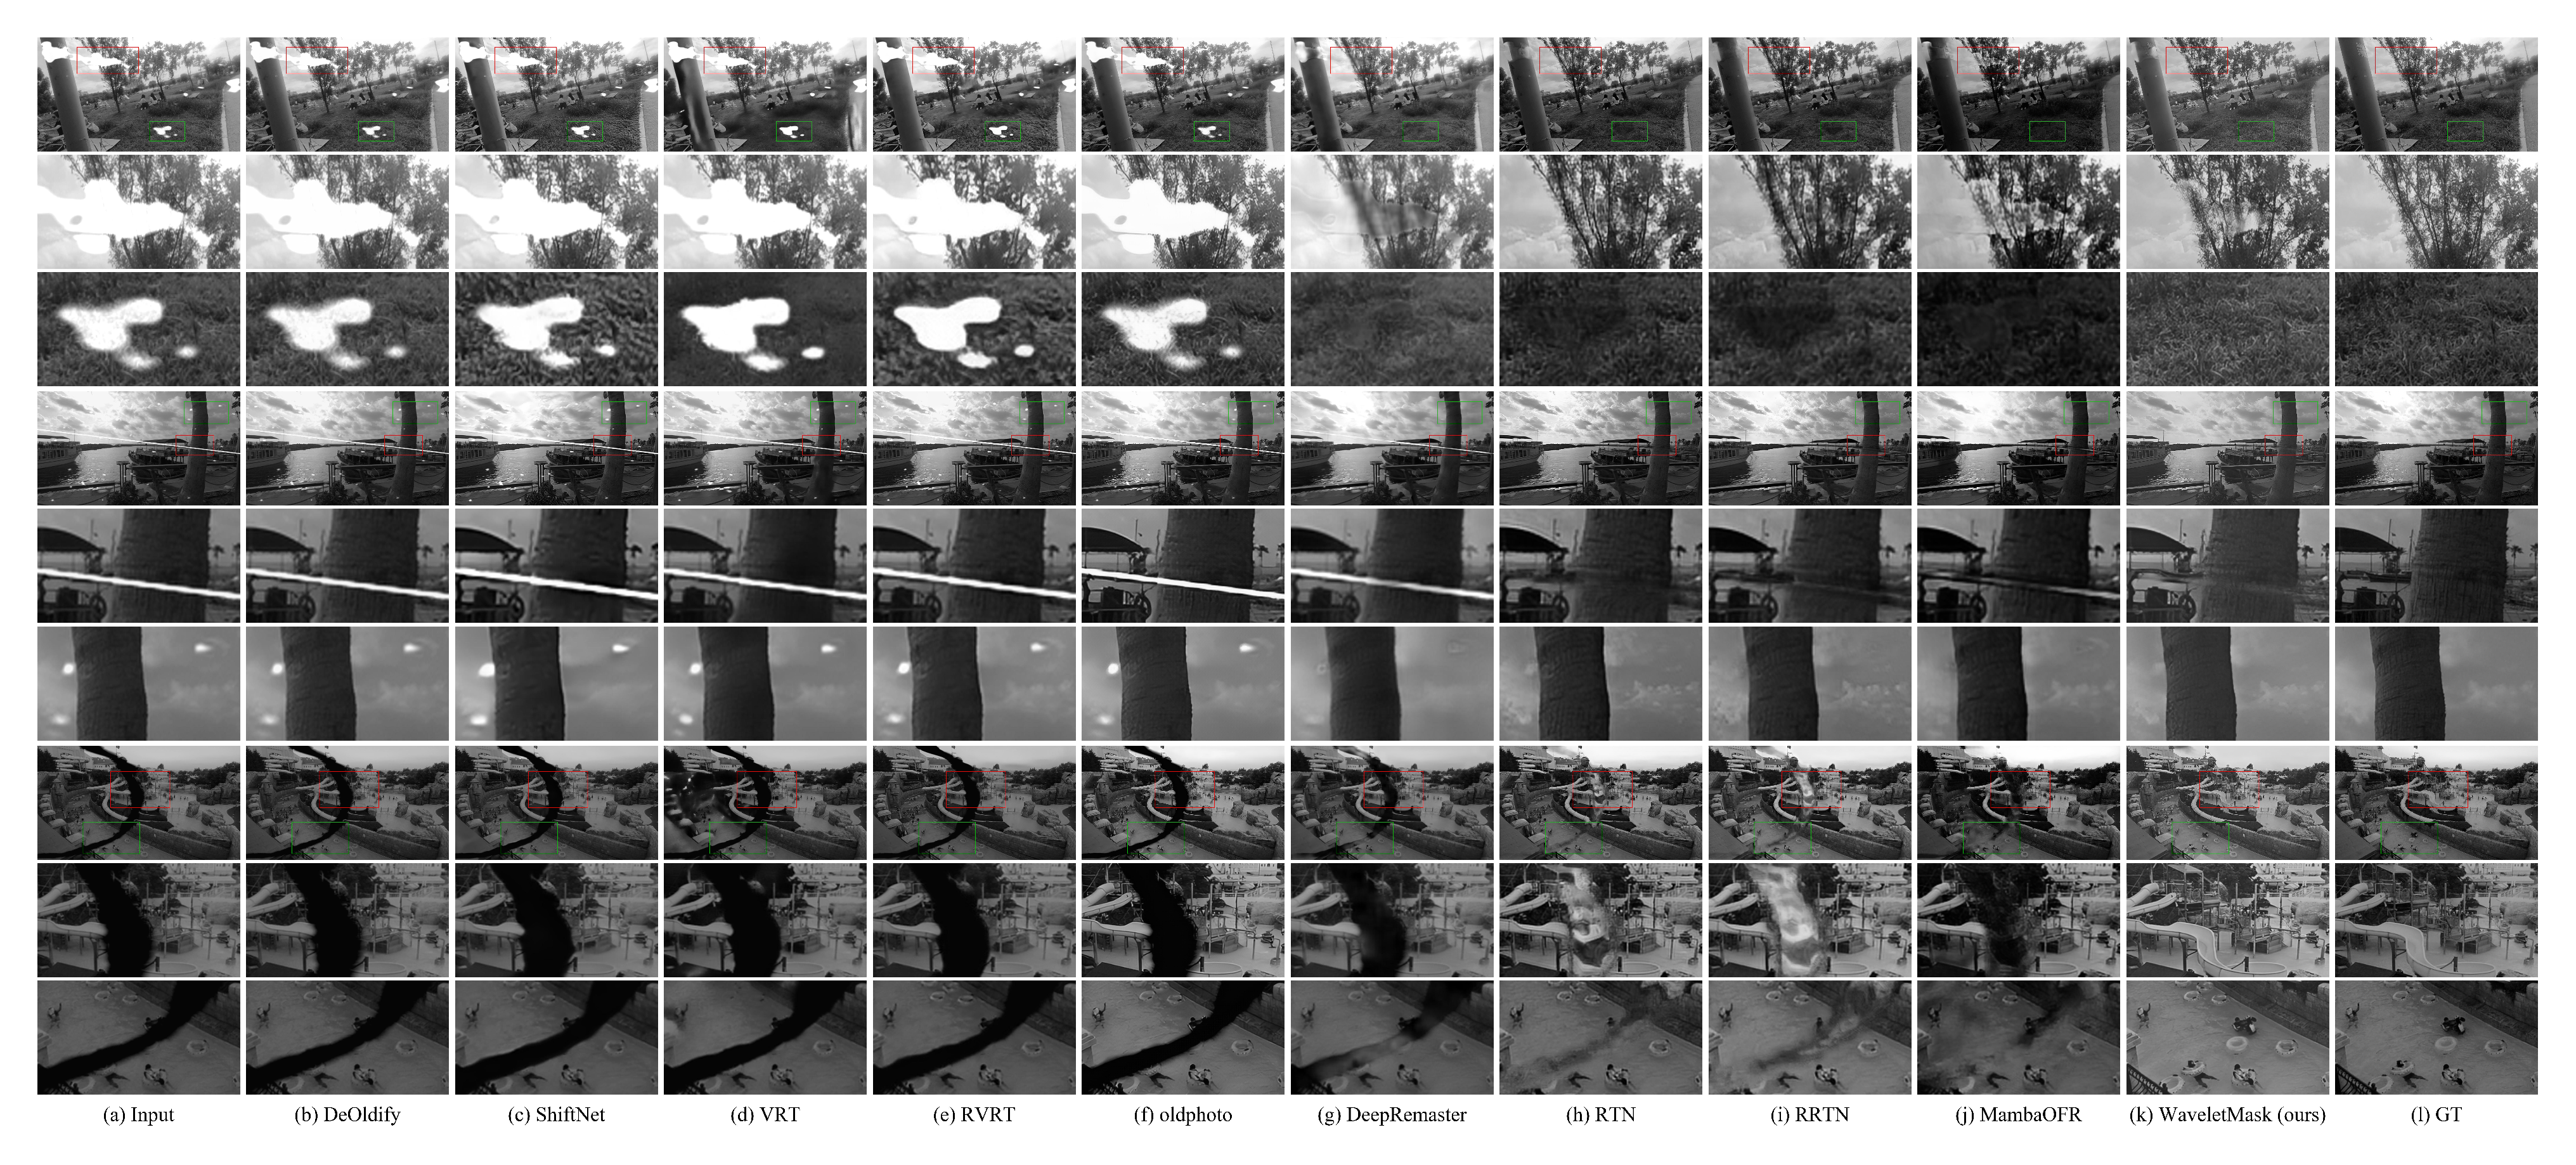
\includegraphics[width=\textwidth]{figures/Figure5.pdf}
\caption{Qualitative comparison on synthetic old-film degradation from the SRWOV/REDS synthetic test setting. Columns: (a) input, (b) DeOldify, (c) ShiftNet, (d) VRT, (e) RVRT, (f) OldPhoto, (g) DeepRemaster, (h) RTN, (i) RRTN, (j) MambaOFR, (k) WaveletMask, and (l) ground truth (GT). ROI crops highlight selected damage regions.\label{fig:sota_synthetic}}
\end{figure}

\begin{figure}[t]
\centering
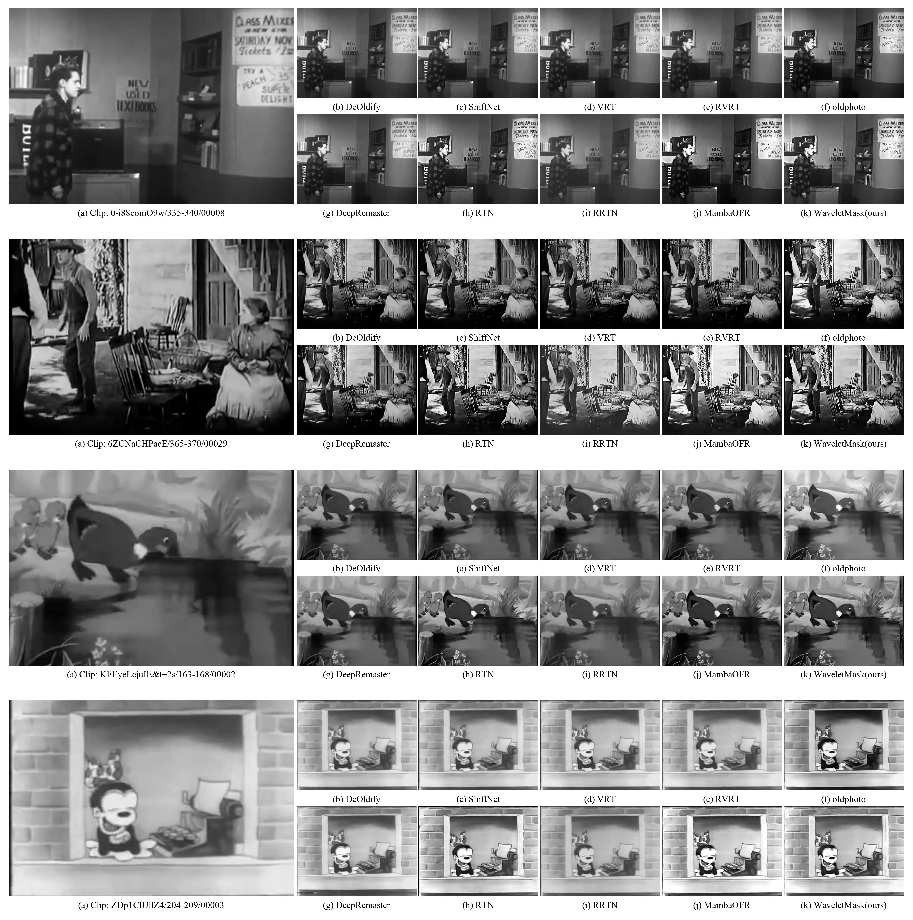
\includegraphics[width=\textwidth]{figures/Figure6.pdf}
\caption{Qualitative comparison on SRWOV real-world archival clips without paired ground truth. Each row compares one input clip/ROI with outputs from (b) DeOldify, (c) ShiftNet, (d) VRT, (e) RVRT, (f) OldPhoto, (g) DeepRemaster, (h) RTN, (i) RRTN, (j) MambaOFR, and (k) WaveletMask. Full-reference scores are unavailable for this split.\label{fig:sota_realworld}}
\end{figure}

Figure~\ref{fig:sota_synthetic} shows representative synthetic examples, where WaveletMask removes scratch and dust residuals more cleanly than the RTN output in the highlighted ROIs. Figure~\ref{fig:sota_realworld} shows the same tendency on archival clips, with cleaner local damage removal and more stable brightness restoration while preserving scene appearance. Spatial error-map analysis confirms that the gains are concentrated in damaged regions (Supplementary Figure~S5). The overall improvement raises the question of whether the gain is uniform across degradation types, which is analyzed in Appendix~\ref{subsec:artifact_breakdown}.

\subsection{Ablation Study}\label{subsec:ablation}

The ablation study is organized around four questions:
\begin{itemize}
\item \textbf{Q1 (Branch effectiveness).} Do LHFM and GFM each improve over the RTN pixel-domain gate, and are the two branches complementary?
\item \textbf{Q2 (Fusion rule).} Is parameter-free branch-level maximum fusion preferable to learned pixel-wise fusion?
\item \textbf{Q3 (Wavelet family).} How sensitive is the gate to the wavelet basis and the number of decomposition levels?
\item \textbf{Q4 (Robustness).} Do the gains persist across artifact types, motion and occlusion levels, and unseen content (Appendix~\ref{app:robustness})?
\end{itemize}

Questions Q1--Q3 are addressed by the three panels of Table~\ref{tab:ablation_core}, while Q4 is examined in Appendix~\ref{app:robustness}. To isolate the contribution of the wavelet-domain branches and the key design choices, Table~\ref{tab:ablation_core} groups three sets of contrasts under the same RTN backbone and training recipe: (a) the detection-branch components (RTN, +LHFM only, +GFM only, and the full WaveletMask variant with branch-level maximum fusion as defined in Equation~\eqref{eq:wavelet_mask}); (b) the key fusion-strategy contrasts between the parameter-free maximum rule and learned CNN fusion; and (c) the key wavelet-family contrasts around the single-level Haar default. The RTN, WaveletMask, and panel (c) rows are measured under the primary Y-channel re-test, whereas the +LHFM only, +GFM only, and learned-fusion rows come from an earlier identical-recipe evaluation run with a slightly different LPIPS/DISTS configuration; the cross-run drift is below 0.002 on these two metrics and does not affect the within-panel ranking.

\begin{table}[H]
\caption{Ablation study on SRWOV synthetic data: panel (a) compares the detection-branch components, panel (b) the proposed branch-level maximum rule against representative learned-fusion variants, and panel (c) representative wavelet families. All variants share the same RTN backbone and training recipe. Within panel (a), best results are in \textcolor{red}{red} and second-best results in \textcolor{blue}{blue}.\label{tab:ablation_core}}
\footnotesize
\begin{tabularx}{\textwidth}{lCCCC}
\toprule
\textbf{Variant} & \textbf{PSNR$\uparrow$} & \textbf{SSIM$\uparrow$} & \textbf{LPIPS$\downarrow$} & \textbf{DISTS$\downarrow$} \\
\midrule
\multicolumn{5}{l}{\textit{(a) Detection-branch components}} \\
RTN     & 26.1648 & 0.8923 & 0.1023 & 0.0946 \\
+LHFM only       & \textcolor{blue}{26.3778} & \textcolor{blue}{0.8966} & \textcolor{blue}{0.0914} & \textcolor{red}{0.0790} \\
+GFM only        & 26.1024 & \textcolor{red}{0.8980} & 0.0969 & 0.0916 \\
\textbf{WaveletMask (max fusion)} & \textcolor{red}{26.6125} & 0.8954 & \textcolor{red}{0.0886} & \textcolor{blue}{0.0827} \\
\midrule
\multicolumn{5}{l}{\textit{(b) Fusion strategy (key contrasts)}} \\
Branch-level maximum (proposed) & 26.6125 & 0.8954 & 0.0886 & 0.0827 \\
Gated CNN fusion & 26.3515 & 0.8966 & 0.0869 & 0.0842 \\
Max + pixel-wise CNN fusion & 24.9827 & 0.8896 & 0.1068 & 0.0867 \\
\midrule
\multicolumn{5}{l}{\textit{(c) Wavelet family (key contrasts)}} \\
Haar, single level (proposed) & 26.6125 & 0.8954 & 0.0886 & 0.0827 \\
Haar, two levels & 26.5175 & 0.9011 & 0.0847 & 0.0760 \\
DTCWT (dual-tree complex) & 26.4506 & 0.8992 & 0.0862 & 0.0780 \\
Daubechies-2 & 17.9208 & 0.6473 & 0.4136 & 0.3154 \\
\bottomrule
\end{tabularx}
\normalsize
\end{table}

Panel (a) of Table~\ref{tab:ablation_core} shows that LHFM alone improves PSNR by $+0.21$~dB over the RTN and yields the lowest DISTS, confirming the value of high-frequency local cues. GFM alone slightly reduces PSNR ($-0.06$~dB) but achieves the best SSIM, indicating stronger structural consistency. The full WaveletMask model reaches 26.61~dB, a $+0.45$~dB gain over RTN and the best LPIPS among the four variants. This is because LHFM targets local scratches and dust, whereas GFM stabilizes low-frequency temporal brightness variation, so their fusion provides complementary guidance. The combined improvement is larger than the arithmetic sum of the individual PSNR changes ($+0.21-0.06=+0.15$~dB), which further supports the complementarity of the two branches.

Panel (b) condenses the fusion-strategy finding: every learned-fusion variant underperforms its direct counterpart in PSNR under the tested recipe (within the fusion-ablation evaluation run, the gated CNN variant trails the maximum rule by 0.25~dB and the max+CNN variant by 1.62~dB), because the compact CNN must fuse heterogeneous sparse cues only through the final restoration loss, making optimization less stable than the parameter-free maximum rule. The gated variant does attain slightly better SSIM and LPIPS than the maximum rule, but it remains behind on PSNR and DISTS, whereas the max+CNN variant is inferior on all four metrics; the parameter-free rule therefore remains the preferred default for the fidelity-oriented design goal. Panel (c) condenses the wavelet-family finding: single-level Haar is the most stable PSNR-oriented default, Haar two-level and DTCWT remain competitive with small PSNR costs and partial perceptual gains, and longer-support wavelets fail catastrophically because filter lengths exceeding two require boundary padding in the wavelet analysis, which introduces border artifacts into the half-resolution sub-band maps processed by the detector heads. The complete fusion comparison, the full wavelet-family and stronger-fusion sweeps, and a cross-domain frequency-operator diagnostic that situates Haar among Sobel/Laplacian, Gaussian-pyramid, Fourier-temporal, and learned shallow alternatives are reported in Appendix~\ref{app:complexity_details} (Tables~\ref{tab:fusion_comparison} and~\ref{tab:followup_ablations}) and Appendix~\ref{app:diagnostics} (Table~\ref{tab:cross_domain_frequency_ablation}).

Figure~\ref{fig:ablation} visually supports the same trend: LHFM mainly removes local scratches, GFM mainly stabilizes frame-level brightness, and the full model combines both effects. Beyond these end-to-end ablations, four detector diagnostic probes confirm that the two branches are complementary rather than redundant and that the fused mask aligns with residual-proxy regions (Appendix~\ref{app:diagnostics}).

\begin{figure}[H]
\centering
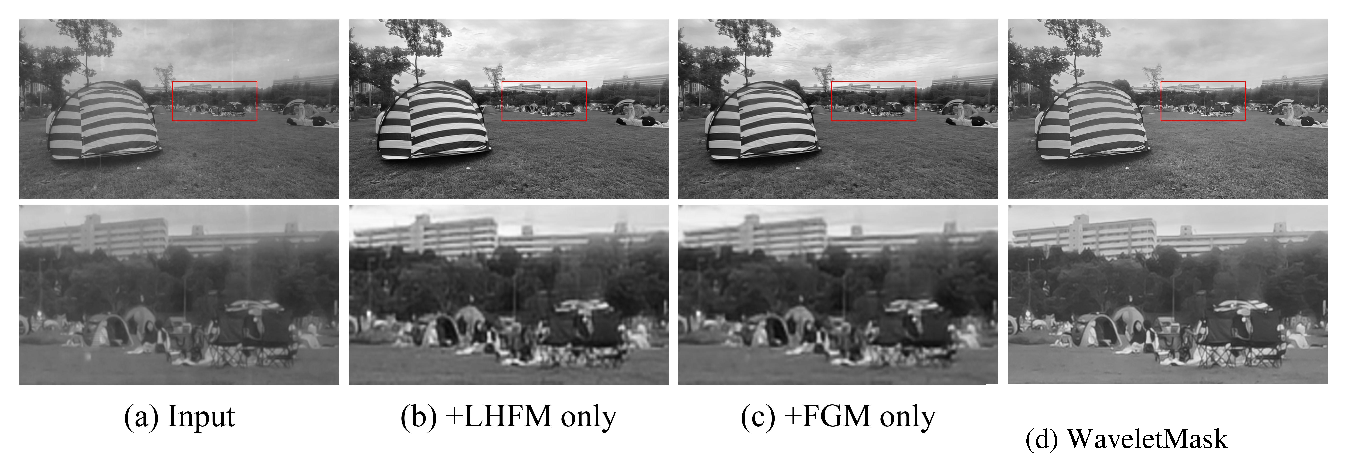
\includegraphics[width=\textwidth]{figures/Figure7.pdf}
\caption{Ablation visual comparison on selected synthetic old-film examples. Columns: (a) degraded input, (b) +LHFM only, (c) +GFM only, and (d) WaveletMask. ROIs mark local damage regions.\label{fig:ablation}}
\end{figure}

\subsection{Computational Complexity}\label{subsec:complexity}

Table~\ref{tab:complexity} summarizes parameters, floating point operations (FLOPs), and runtime cost. We report these figures to make the cost of the proposed detector explicit rather than to claim minimum latency. All rows are measured by us under one unified protocol on the same device, so the comparison is consistent across methods; the deployment-relevant quantity is the overhead that the proposed gate adds to its host network.

\begin{table}[H]
\caption{Computational cost measured by us under one unified protocol on a single NVIDIA L40 GPU in FP32 (batch size 1, seven-frame $256\times256$ clips, three warm-up and ten timed runs). Parameters and FLOPs cover the full executable forward pass on a $1\times7\times3\times256\times256$ input and include the RAFT flow estimator for the flow-based methods (RTN, RRTN, MambaOFR, WaveletMask); DeepRemaster uses no flow estimator. Latency is reported per seven-frame clip. The measurement protocol and additional batch/resolution settings are detailed in Appendix~\ref{app:complexity_details}.\label{tab:complexity}\label{tab:runtime_benchmark}}
\footnotesize
\begin{tabularx}{\textwidth}{lCCCCC}
\toprule
\textbf{Method} & \textbf{Params (M)} & \textbf{FLOPs (G)} & \textbf{Latency (ms/clip)$\downarrow$} & \textbf{Throughput (fps)$\uparrow$} & \textbf{Peak Mem. (GB)$\downarrow$} \\
\midrule
DeepRemaster~\cite{iizuka2019deepremaster}  & 9.8781 & 914.0  & 17.9  & 391.6 & 0.35 \\
RTN~\cite{rtn2022}                          & 5.7351 & 2184.7 & 169.5 & 41.3  & 0.24 \\
RRTN~\cite{rrtn2024}                        & 7.0503 & 2782.2 & 298.4 & 23.5  & 0.75 \\
MambaOFR~\cite{mao2025mambaofr}             & 8.2984 & 2832.8 & 404.8 & 17.3  & 0.60 \\
\midrule
WaveletMask                                 & 5.7360 & 2184.9 & 171.4 & 40.8  & 0.24 \\
\bottomrule
\end{tabularx}
\normalsize
\end{table}

The proposed detector adds 898 learnable parameters and 0.1494G FLOPs to the RTN, with nearly identical latency (171.4 vs.\ 169.5~ms per clip) and identical peak memory. At $1280\times720$, batch-size-1 inference takes about 5.4~s per seven-frame clip with 9.9~GB peak memory for both models, so WaveletMask inherits the cost profile of its backbone and is not yet real-time at high resolution in FP32. The full measurement protocol, additional batch and resolution settings, and the per-module parameter breakdown of the detection pathway are provided in Appendix~\ref{app:complexity_details} (Table~\ref{tab:module_overhead}).
